%Sample usage of usuthesis.cls
\documentclass[ee, msthesis]{usuthesis}

%{{{ Some useful packages, modify as needed
\usepackage{epsfig}
\usepackage{amssymb}           % add ams symbols stuff
\usepackage{amsmath}
\usepackage{amsthm}
\usepackage{mathtools }
\usepackage{caption}		% needed for listing captions
\usepackage{subcaption}
\usepackage{graphicx}          	% add graphics
\usepackage{tikz,pgfplots}
\usepackage{gincltex}
\usepackage{color}             	% grants control of link text colors.
\usepackage[linesnumbered,lined,boxed,ruled,commentsnumbered]{algorithm2e}
\usepackage{setspace}
\usepackage{listings}		% code listings
\usepackage{pdflscape}
\usepackage{hyperref}          	% make contents/ref/citations clickable
\usepackage{epstopdf}
\usepackage{enumerate}		% lists of items
\usepackage{url} 			% url in bib

%}}}

% for formatting code
\lstset{
	language=Python,                		% choose the language of the code
	basicstyle=\footnotesize,       		% the size of the fonts that are used for the code
	numbers=left,                   		% where to put the line-numbers
	numberstyle=\footnotesize,		% the size of the fonts that are used for the line-numbers
	stepnumber=1,                   		% the step between two line-numbers. If it is 1 each line will be numbered
	firstnumber=100,
	lineskip={5pt},
	aboveskip={2\baselineskip},
	belowskip={0\baselineskip},
	xleftmargin=0mm,				% left margin of listing section
	floatplacement=t,
	numbersep=-15pt,                  	% how far the line-numbers are from the code
	backgroundcolor=\color{white},  	% choose the background color. You must add \usepackage{color}
	showspaces=false,               		% show spaces adding particular underscores
	showstringspaces=false,         	% underline spaces within strings
	showtabs=false,                 		% show tabs within strings adding particular underscores
	frame=tb,           				% adds a frame around the code
	tabsize=4,          				% sets default tabsize to 2 spaces
	captionpos=b,           			% sets the caption-position to bottom
	breaklines=true,        			% sets automatic line breaking
	breakatwhitespace=false,    		% sets if automatic breaks should only happen at whitespace
	numberbychapter=true,
	escapeinside={\%*}{*)}          		% if you want to add a comment within your code
}
\lstloadlanguages{
         Java,HTML,Python
 }

\intextsep=10mm					% controls spacing before and after figures and tables
\belowcaptionskip=-5mm

%Set all linked content to be plain black text
\hypersetup{
    colorlinks,%
    citecolor=black,%
    filecolor=black,%
    linkcolor=black,%
    urlcolor=black
}

\newtheorem{theorem}{Theorem}

\DeclarePairedDelimiter\abs{\lvert}{\rvert}%
\DeclarePairedDelimiter\norm{\lVert}{\rVert}%

% Author and Title Information
\author{Alexandros D. Keros}
\title{Scaling Geometric Monitoring over Distributed Streams}


% The Committee
\majorprof{Dr. Vasilis Samoladas}
\firstreader{first reader}
\secondreader{second reader}
%Dissertation includes additional committee members
%\thirdreader{}
%\fourthreader{}

% Graduate Dean, Update as necessary
\graddean{dean} 
\deantitle{}
\deansecondtitle{}

% Degree Information
\degree{Undergraduate}
\month{September}
\myyear{2015}
\university{Technical University of Crete}

\begin{document}

    %{{{ Frontmatter
    \preliminaries   % set frontmatter style

    \maketitle
    \makecopyright        % optional

    \begin{abstract}

Modern applications, such as telecommunication and sensor networks, have brought distributed data streams to the foreground, with monitoring tasks being an important aspect of such systems. The inefficiency of collecting data to a central point for processing dictates the need to devise local or semi-local algorithms that aim to reduce the communication overhead while retaining accuracy standards. 

The \emph{geometric monitoring method} [Sharfman et al., ``A Geometric Approach to Monitoring Threshold Functions over Distributed Data Streams'', ACM SIGMOD '06 ICMD] provides a framework for enforcing local constraints at distributed nodes, as well as a method for resolving violations not representing the system's state i.e., false alarms, in order to reduce the necessary communication with the coordinating node. Furthermore, successive work proposed optimizations to the selection process of the nodes participating to the set that resolves such violations. 

We propose a heuristic method that exploits data stream characteristics and utilizes multi-objective optimization in order to avert, or delay, successive false alarms by optimally positioning vector representations of data streams during the violation resolution process. Additionally, a hierarchical node clustering method for deterministic and optimal node selection, found in [ Keren et al., ``Geometric Monitoring of Heterogeneous Streams'', IEEE Trans. Knowl. Data Eng., 2014], is improved and simplified. Extensive experimentation on real-world and synthetic datasets showcase that the proposed methods can reduce the communication burden in half, compared to that of the original geometric monitoring method.

\end{abstract}
    \begin{publicabstract}

BLAH BLAH

\end{publicabstract}
    \include{doc/dedication}  % optional
    \begin{acknowledgments}

my mum 

\end{acknowledgments}     % optional

    \tableofcontents
    \listoftables
    \listoffigures

%    \include{doc/notation}  % optional
%    \include{doc/acronyms}  % optional
    %}}}
    %{{{ The main body of the thesis
    \body  % set main body style

    % Chapters
    %part
	\part{INTRODUCTION AND PRELIMINARIES} \label{pt:introPrelim}    
    \chapter{Introduction} \label{chap:intro}
\section{Overview} \label{sec:intro-overview}


A multitude of recent emergent applications require real-time handling of rapidly incoming data, that may as well be great in size and distributed in nature. Such applications that follow a continuous distributed monitoring model are classified as \emph{Data Stream Systems}~\cite{Babcock2002DataStreamSystems}. Notable examples include, among others, distributed sensors, ISP network traffic monitoring, telecommunication system management, event monitoring, and real-time analysis tools for financial data.

These systems differ from the traditional Database Management Systems (DBMS), in the sense that they are following a \emph{pull paradigm}, where large scale event monitoring is required or continuous queries are issued, instead of the \emph{push paradigm}, where one-shot queries normally take place. Data Stream Systems are required to efficiently process, in real-time, data streams that are of high volume, continuous, size unbound, and most likely violative, in the sense that it would be inefficient to store them in memory. Additionally, the distributed nature of some applications incur an additional challenge to such systems, for they are required to communicate via a bandwidth-limited and possibly delay-inducing network in order to synchronize, reorganize, and provide a real-time overview of the results.

Consequently, intelligent algorithms must be devised that are able to guarantee high accuracy standards while limiting the communication overhead induced to the distributed setting. Approaches such as collecting all data to a central node for processing and polling nodes for data updates, as easily implementable as they may be, are prohibitive is such a decentralized scenario, either due to the communication and storage overhead they induce, or due to the accuracy degradation they inflict. 

The geometric monitoring method proposed by Sharfman et al.~\cite{Sharfman2006GM} consists of a geometric approach in which convex optimization theory is being employed in order to guarantee that communication between distributed nodes takes place only when needed, while maintaining strict bounds on the accuracy of the monitoring task. By decomposing the task to local constraints at the  nodes, and by employing a clever mechanism for resolving constraint violations that are not representative of the system's state, i.e. false alarms, the communication between sites is significantly reduced without any accuracy degradation.

Following this framework, much work has emerged attempting to improve the communication bounds of the geometric monitoring method and to generalize the method to applications in the likes of continuous query answering. Following this trend, this thesis employs heuristics structured on top of multi-objective optimization problems and signal processing filters in order to better the performance of the geometric monitoring algorithm. Additionally, an existing method for hierarchical clustering of distributed streams, found in~\cite{Sharfman2012ShapeSensGM}, is improved and simplified.

Evaluation of the proposed algorithms over synthetic and real-world datasets exhibits an improvement of up to 60\% over the original geometric monitoring method. Furthermore, the behaviour of the proposed algorithms in different settings is being researched.


\section{Motivation} \label{sec:intro-motivation}

A lot of work towards this direction, based on GM.
We believe that there is still room for improvements regarding the way the method handles and represents data streams

\section{Contributions} \label{sec:intro-contr}

\section{Thesis Outline} \label{sec:intro-thesisOutline}
     \chapter{Theoretical Background} \label{chap:theorBack}

The present chapter contains the background knowledge required throughout the length of this thesis. Section~\ref{sec:theorBack-GM} describes the framework of the \emph{Geometric Monitoring method}. Section~\ref{sec:theorBack-MOP} presents \emph{multi-objective optimization} and  dives into the algorithms used in our implementation. Section \ref{sec:theorBack-MWMGraphs} discusses \emph{graph maximum weight matching}, and, finally, in Section~\ref{sec:theorBack-SavitzkyGolay} we explain the \emph{Savitzky-Golay filtering} used for smoothing, velocity and acceleration approximation.

%TODO gaussian process and lwpr?

\section{Geometric Monitoring of Distributed Streams} \label{sec:theorBack-GM}
 
The \emph{Geometric Monitoring} method~\cite{Sharfman2006GM} was devised as a way to monitor threshold crossings of arbitrary functions over distributed data streams, i.e. be able to determine whether an arbitrary \emph{monitoring function} $f(\cdot)$ over the data streams violated a predetermined threshold ($f(\cdot)>T$ or $f(\cdot)<T$). By mapping data streams to a feature space defined by the dimensionality of each data stream update and monitoring the convex hull surrounding the value of the monitoring function, Sharfman et al. were able to decompose the monitoring task into local constraints and apply distributed threshold monitoring, while reducing the communication costs required by central data processing.

In the current section a detailed presentation of this method is taking place. In Subsection~\ref{subsec:theorBack-GM-sysArch} two system architectures are shown, a decentralized scenario and a centralized one, where Geometric Monitoring can be applied. Subsection~\ref{subsec:theorBack-GM-compMod} explains the computational model, followed by the method's geometric interpretation in Subsection~\ref{subsec:theorBack-GM-geomInt}. Finally, in Subsection~\ref{subsec:theorBack-GM-protocol} the protocol implementing the Geometric Monitoring method is described.


\subsection{System Architecture} \label{subsec:theorBack-GM-sysArch}

In~\cite{Sharfman2006GM} two different scenarios of Geometric Monitoring corresponding to different network topologies are examined. The \emph{decentralized scenario} refers to a topology where nodes are allowed to communicate with each other and a central node is absent. The \emph{centralized scenario} models a star network topology, where a coordinator node communicating with all other nodes is existent.

\subsubsection{Decentralized Scenario} \label{subsubsec:theorBack-GM-decentralized}

The topology examined is that of a partially or fully connected mesh network where a coordinator node is absent and nodes are allowed to broadcast to the network or communicate with each other according to the links existent between them. Data stream update vectors arrive continuously at each of the monitoring nodes and nodes must always be synchronized, i.e. all nodes must be aware of the monitoring task's state at all times. An example is depicted in Figure~\ref{fig:decentralized}.

%%%%%%%%%%%%%%%%%%%%%%%%%%%%%%%%%%%% decentralized figure %%%%%%%%%%%%%%%%%%%%%%%%%%%%%%%%%%%%
\begin{figure}[H]
\centering
\includegraphics{img/decentralized.tex}
\caption{Network topology example of the decentralized scenario. Dashed lines represent data streams and half arrows represent message exchanges.} 
\label{fig:decentralized}
\end{figure}
%%%%%%%%%%%%%%%%%%%%%%%%%%%%%%%%%%%%%%%%%%%%%%%%%%%%%%%%%%%%%%%%%%%%%%%%%%%%%%%%%%%%%%%%%%%

\subsubsection{Centralized Scenario}\label{subsubsec:theorBack-GM-centralized}

The \emph{centralized}, or \emph{coordinator-based} scenario is built upon a star network topology, where all monitoring nodes communicate with a central node, the \emph{coordinator node}. Nodes receive data stream update vectors continuously, and must communicate their state information to the coordinator node when needed. The coordinator receives data stream updates as well, which can be modelled by an additional monitoring node responsible for the cooridinator node's data stream. Communication between monitoring nodes is not allowed, thus, only the communicator can, and must, be aware of the state of the monitoring task at all times. An example is depicted in Figure~\ref{fig:centralized}.

%%%%%%%%%%%%%%%%%%%%%%%%%%%%%%%%%%%% centralized figure %%%%%%%%%%%%%%%%%%%%%%%%%%%%%%%%%%%%
\begin{figure}[H]
\centering
\includegraphics{img/centralized.tex}
\caption{Network topology example of the centralized scenario.The bold node represents the coordinator node. Dashed lines represent data streams and half arrows represent message exchanges.} 
\label{fig:centralized}
\end{figure}
%%%%%%%%%%%%%%%%%%%%%%%%%%%%%%%%%%%%%%%%%%%%%%%%%%%%%%%%%%%%%%%%%%%%%%%%%%%%%%%%%%%%%%%%%%%

\subsection{Computational Model} \label{subsec:theorBack-GM-compMod}

The main goal of the Geometric Monitoring method is to efficiently detect threshold crossings of an arbitrary function over distributed data streams. This is realized via vector projections of the data streams and convex local constraint assignments regarding said vectors at the nodes.

Let $f:\mathbb{R}^d \to \mathbb{R}$ be an arbitrary function, the \emph{monitoring function}, whose value over the data streams needs to be monitored, so that if $f(\cdot)>T$ or $f(\cdot)<T$ an alarm is raised. For linear functions this problem is trivial, so that by letting, for example, $x_1$ and $x_2$ be data stream values at different nodes and requiring $f(\frac{x_1+x_2}{2})>10$ to be monitored, it holds that $f(\frac{x_1+x_2}{2})=\frac{f(x_1)+f(x_2)}{2}$, and the problem can be decomposed to local constraints $f(x_i)<10, i=1,2$ at both nodes, i.e. a node remains silent until it violates its local constraint. Consider now the case of a non-linear function. By knowing the value of the function at the nodes nothing can be deduced about the function's value over the average of the monitoring streams and where it is positioned with respect to the threshold. Let $f(x)=10x-x^2$, $x_1=0$ and $x_2=9$. Even thought $f(x_1)=0<10$ and $f(x_2)=9<10$, their average violates the specified threshold, $f(\frac{x_1+x_2}{2})=f(4.5)=24.75>10$. 

In order to be able to effectively track non-linear functions, in the likes of the aforementioned example, a mapping of the streams to a vector space is taking place. Let $P=\{p_1, \dots, p_n\}$ be the monitoring node set with weights $w_1, \dots, w_n$, which can be either static or time varying. Their respective data streams $S=\{s_1, \dots, s_n\}$ are represented by $\vec{v_1}(t), \dots, \vec{v_n}(t)$, the $d$-dimensional \emph{local statistics vectors} of the nodes at time $t$. The \emph{global statistics vector} at time $t$ is the weighted average of the local statistics vectors, as such:
\begin{equation}
\vec{v}(t)=\frac{\sum_{i=1}^n{w_i\vec{v_i}(t)}}{\sum_{i=1}^n{w_i}}
\label{form:globalStatsVector}
\end{equation}

Infrequent communication between monitoring nodes, in the decentralized scenario, or between monitoring nodes and the coordinator, in the coordinator-based scheme, dictates the need to keep track of the value of the global statistics vector at the time the last global communication occurred, thus forming the \emph{estimate vector}:
\begin{equation}
\vec{e}(t)=\frac{\sum_{i=1}^n {w_i \vec{v_i}'}}{\sum_{i=1}^n {w_i}}
\label{form:estimateVector}
\end{equation}
,where $\vec{v_i}'$ is the last communicated statistics vector of node $p_i$.

At the monitoring nodes the difference between the current local statistics vector and the last communicated statistics vector is denoted by $\Delta \vec{v_i}(t)=\vec{v_i}(t)-\vec{v_i}', i=1,\dots,n$. The \emph{drift vector} $\vec{u_i}(t), i=1,\dots,n$, also maintained at the monitoring nodes, represents the deviation of each node's data stream from the estimate vector and is defined differently in the two scenarios:
\begin{itemize}
\item In the \textbf{decentralized} setting the drift vector is regarded as the displacement of the local statistics vector from the estimate vector:
\begin{equation}
\vec{u_i}(t)=\vec{e}(t)+\Delta \vec{v_i}(t)
\label{form:decentralizedDrift}
\end{equation}
\item In the \textbf{centralized} setting the monitoring nodes forward their state to the coordinator node, who has a global overview of the monitoring task at hand. This property allows the coordinator to counteract the effects a specific stream has on the partially observed monitoring task with an other, ``opposite'', stream belonging to a different monitoring node. This is taken care by the \emph{balancing process} initiated every time a local violation occurs, which is responsible for computing and communicating the \emph{slack vector} $\vec{\delta_i}$ to the nodes that contributed to the process, thus providing them with the necessary disposition of their drift vectors, as such:
\begin{equation}
\vec{u_i}(t)=\vec{e}(t)+\Delta \vec{v_i}(t)+\frac{\vec{\delta_i}}{w_i}
\label{form:centralizedDrift}
\end{equation} 
\end{itemize}

\subsubsection{Balancing Process} \label{subsubsec:theorBack-GM-balancingProc}

The balancing process taking place in the \textbf{centralized scenario} is initiated by the coordinator node every time a threshold violation occurs, with the objective of resolving a possibly false alarm with minimal communication overhead. This task is executed by collecting a subset of monitoring nodes' data, the \emph{balancing set} $P'$, until the average of their drift vectors, the \emph{balancing vector}, does not cause a threshold crossing. The balancing vector is formulated as follows:
\begin{equation}
\vec{b}=\frac{ \sum_{p_i \in P'} {w_i\vec{u_i}(t)} }{ \sum_{p_i \in P'} {w_i} }
\label{form:balancingVector}
\end{equation}

After a successful balancing process has come to an end, $\Delta\vec{\delta_i}$ slack vector adjustments for all participants in the balancing set $P'$ are computed and communicated to their respective sites, so that local drift vectors can be readjusted to reflect the balancing operation by computing $\vec{\delta_i}=\vec{\delta_i}'+\Delta\vec{\delta_i}$, where $\vec{\delta_i}'$ the previous slack vector (Equation~\ref{form:centralizedDrift}). These adjustments are calculated as follows:
\begin{equation}
\Delta\vec{\delta_i}=w_i\vec{b}-w_i\vec{u_i}(t)\ \forall\ p_i \in P'
\end{equation}
, where $\sum_{p_i \in P'} \Delta \vec{\delta_i}= \vec{0}$. Once the slack vector adjustments have been communicated to the respective monitoring nodes participating in $P'$, their drift vectors are essentially set to the value of the newly computed balancing vector.

In case the balancing process proves unsuccessful all monitoring nodes are contained in the balancing set $P'$ and a new estimate vector is computed with the data cumulated at the coordinator node. Subsequently, all drift vectors and slack vectors are set to $\vec{0}$.

\subsection{Geometric Interpretation} \label{subsec:theorBack-GM-geomInt}

The estimate vector, being the product of the system's previous global synchronization, is known to all monitoring nodes and denotes the last known position of the global statistics vector. That being said, the estimate vector is considered valid if it resides on the same side of the threshold as the unknown global statistics vector.
In order to estimate the current position of the global statistics vector, since a mere observation of the monitoring function's value at each stream provides no information about its current location (as described in Section~\ref{subsec:theorBack-GM-compMod}), it is vital that the task is decomposed into local constraints that will guarantee the timely detection of a violation of the estimate's vector validity.

The \emph{convexity property} of the drift vectors, along with Theorem~\ref{theorem:convexHull}~\cite{Sharfman2006GM}, are sufficient in provide a framework for decomposing the monitoring task into local constraints at the nodes. Both the convexity property and the relevant theorem are repeated below for completeness.
	
The convexity property dictates that the weighted average of the drift vectors equal the global statistics vector, as such:
\begin{equation}
\vec{v}(t)=\frac{\sum_{i=1}^n {w_i\vec{u_i}(t)}}{\sum_{i=1}^n {w_i}}
\label{form:convexityProperty}
\end{equation}
The geometric interpretation of the property guarantees that the global statistics vector $\vec{v}$ is always contained in the convex hull defined by the drift vectors $\vec{u_i}, i=1,\dots,n$.


\begin{theorem}[Sharfman et al.~\cite{Sharfman2006GM}]\label{theorem:convexHull}
Let $\vec{x}, \vec{y_1}, \dots, \vec{y_n} \in \mathbb{R}^d$ be a set of vectors in $\mathbb{R}^d$. Let $Conv(\vec{x}, \vec{y_1}, \dots, \vec{y_n})$ be the convex hull of $\vec{x}, \vec{y_1}, \dots, \vec{y_n}$. Let $B(\vec{x}, \vec{y_i})$ be a ball centered at $\frac{\vec{x}+\vec{y_i}}{2}$ and with radius of $\norm{\frac{\vec{x}+\vec{y_i}}{2}}_2$ i.e., $B(\vec{x}, \vec{y_i})=\{\vec{z}\ |\ \norm{\vec{z}-\frac{\vec{x}+\vec{y_i}}{2}}_2 \leq \norm{\frac{\vec{x}+\vec{y_i}}{2}}_2 \}$, then $Conv(vec{x}, \vec{y_1}, \dots, \vec{y_n}) \subset B(\vec{x}, \vec{y_i})$.
\end{theorem}

Essentially, Theorem~\ref{theorem:convexHull} states that $n$ $d$-dimensional spheres defined by $n+1$ vectors can effectively bound the convex hull defined by said vectors, as such: $Conv(\vec{x}, \vec{y_1}, \vec{y_2}, \dots, \vec{y_n}) \subset  \cup B(\vec{x}, \vec{y_i}), i=1,\dots,n$, which finds direct application to the distributed monitoring task if $\vec{x}=\vec{e}$ and $\vec{y_i}=\vec{u_i}, i=1,\dots,n$. An example is depicted in Figure~\ref{fig:convexHull}
.


%%%%%%%%%%%%%%%%%%%%%%%%%%%%%%%%%%%% convex hull figure %%%%%%%%%%%%%%%%%%%%%%%%%%%%%%%%%%%%
\begin{figure}[H]
\centering
\includegraphics[scale=0.7, trim=0 0 4.2cm 0]{img/convex_hull.tex}
\caption{Example of a convex hull (light gray) defined by the drift vectors $\vec{u_i}, i=1,2,3,4,5$. The hull is bounded by the spheres created from the estimate vector $\vec{e}$ and the drift vectors $\vec{u_i}, i=1,2,3,4,5$. The global statistics vector $\vec{v}$ is guaranteed to be contained in the convex hull of the drift vectors.} 
\label{fig:convexHull}
\end{figure}
%%%%%%%%%%%%%%%%%%%%%%%%%%%%%%%%%%%%%%%%%%%%%%%%%%%%%%%%%%%%%%%%%%%%%%%%%%%%%%%%%%%%%%%%%%%

\subsubsection{Local Constraints} \label{subsubsec:theorBack-GM-localConstraints}

The decomposition of the threshold monitoring task to local constraints at the nodes, in which each node monitors its respective bounding sphere $B(\vec{e}, \vec{u_i}), i=1,\dots n$ for a possible threshold violation, induces a coloring upon the spheres. Let $V=\{\vec{x} | f(\vec{x}>T)\}$ be the set of vectors said to be \emph{green}, and $\overline{V}=\{\vec{y} | f(\vec{y}<T)\}$ the \emph{red} set of vectors, then the local constraint monitoring at the nodes is essentially a process of monitoring the monochromaticity of a node's bounding sphere $B(\vec{e}, \vec{u_i})$ i.e., all vectors in the bounding ball are of the same color. As long as this monochromaticity is upheld for the whole of the node set, the convex hull defined by the drift vectors is monochromatic and, by the convexity property, the global statistics vector has not crossed the threshold. In case a single node signals a threshold crossing a \emph{local violation} has occurred. If the local violation coincides with a threshold crossing of the global statistics vector, then a \emph{global violation} has occurred.

\subsection{Protocol} \label{subsec:theorBack-GM-protocol}

Two variants of a network's topological structure have been proposed for application of the Geometric Monitoring method, a decentralized scenario and a centralized, coordinator-based one (Section~\ref{subsec:theorBack-GM-sysArch}). The following paragraphs present the algorithms for each of these systems.

\subsubsection{Decentralized Algorithm} \label{subsubsec:theorBack-GM-decentralizedAlgo}

The decentralized scenario of the geometric monitoring method, summarized in Algorithm~\ref{algo:decentralized}, operates on the mesh network described in Section~\ref{subsubsec:theorBack-GM-decentralized}. Each node $p_i$ keeps track of its drift vector $\vec{v_i}(t)$ and the previously communicated statistics vectors $\vec{v_j}'$ from all other nodes $p_j$, from which the estimate vector is locally computed. At the occurence of a local violation the violating node initiates a global system synchronization by broadcasting its local statistics vector along with its unique identifier, from which the estimate vector is globally updated so that monochromaticity checks are valid.\\ 

%%%%%%%%%%%%%%%%%%%%%%%%%%%%%%%%%%%%%%%% decentralized algo %%%%%%%%%%%%%%%%%%%%%%%%%%%%%%%%%%%%%%%%%%%
\begin{algorithm}[H]
\setstretch{1.30}


\Begin{
	\ForEach(\tcc*[f]{Node initialization}){node $p_i$}{
		Broadcast $\vec{v_i}(0)$\;
		$\vec{v_i}'=\vec{v_i}(0)$\;
		Wait messages from all other nodes\;
		\If{messages from all vectors received}{
			$\vec{e}(t)=\frac{\sum_{i=1}^n {w_i \vec{v_i}'}}{\sum_{i=1}^n {w_i}}$\;
		}
	}

	\ForEach(\tcc*[f]{Main monitoring task}){node $p_i$}{
		\ForEach{new $s_i$ stream update $\vec{v_i}(t)$}{
			Recalculate $\vec{u_i}(t)=\vec{e}(t)+\Delta \vec{v_i}(t)$\;
			\If{$B(\vec{e},\vec{u_i}(t))$ is \emph{not} monochromatic}{
				Broadcast message $<i,\vec{v_i}(t)>$\;
				Set $\vec{v_i}'=\vec{v_i}(t)$\;
			}
		

			\If{new message $<j,\vec{v_j}(t)>$ received}{
				Set $\vec{v_j}'=\vec{v_j}(t)$\;
				Recalculate $\vec{e}(t)=\frac{\sum_{i=1}^n {w_i \vec{v_i}'}}{\sum_{i=1}^n {w_i}}$\;
				\If{$B(\vec{e},\vec{u_i}(t))$ is \emph{not} monochromatic}{
					Broadcast message $<i,\vec{v_i}(t)>$\;
					Set $\vec{v_i}'=\vec{v_i}(t)$\;
				}
			}
		}

	}
}
\caption{Decentralized algorithm \label{algo:decentralized}} 
\end{algorithm}
%%%%%%%%%%%%%%%%%%%%%%%%%%%%%%%%%%%%%%%%%%%%%%%%%%%%%%%%%%%%%%%%%%%%%%%%%%%%%%%%%%%%%%%%%%%%%%%%%%%%%%%%%%%%%%%


\subsubsection{Centralized Algorithm} \label{subsubsec:theorBack-GM-centralizedAlgo}

The centralized, coordinator-based geometric monitoring operation is summarized in Algorithms~\ref{algo:centralizedMonitoringNode},  and~\ref{algo:centralizedCoordinatorNode}, where the execution sequence of the monitoring nodes and the execution sequence of the coordinator node are described, respectively. The topology is that of a star network, where nodes are allowed to communicate exclusively with the coordinator node, as described in Section~\ref{subsubsec:theorBack-GM-centralized}. The coordinator node is responsible for answering queries about the monitoring status i.e., has absolute knowledge about threshold violations, and handles the balancing process (Section~\ref{subsubsec:theorBack-GM-balancingProc}). Local streams are tracked by the monitoring nodes on the basis of the last communicated estimate vector, and must inform the coordinator for any local threshold violation. The coordinator node can also monitor is respective data stream without any change in the described framework.\\

%%%%%%%%%%%%%%%%%%%%%%%%%%%%%%%%%%%%%%%% centralized monitoring node algo %%%%%%%%%%%%%%%%%%%%%%%%%%%%%%%%%%%%%%%%%%%
\begin{algorithm}[H]
\setstretch{1.30}
\Begin{
	\ForEach(\tcc*[f]{Node initialization}){node $p_i$}{
		Send $<INIT,\vec{v_i}(0)>$ message to coordinator\;
		$\vec{v_i}'=\vec{v_i}(0)$\;
		$\vec{\delta_i}=\vec{0}$\;
		Wait message from coordinator\;
		\If{$<NEW\textnormal{-}EST, \vec{e}>$ message received}{
			Set $\vec{e}(t)=\vec{e}$\;
		}
	}

	\ForEach(\tcc*[f]{Main monitoring task}){node $p_i$}{
		\ForEach{new $s_i$ stream update $\vec{v_i}(t)$}{
			Recalculate $\vec{u_i}(t)=\vec{e}(t)+\Delta \vec{v_i}(t)+\frac{\vec{\delta_i}}{w_i}$\;
			\If{$B(\vec{e},\vec{u_i}(t))$ is \emph{not} monochromatic}{
				Send $<REP,\vec{v_i}(t),\vec{u_i}(t)>$ message to coordinator\;
				Wait for $<NEW\textnormal{-}EST,\cdot>$ or $<ADJ\textnormal{-}SLK,\cdot>$ message from coordinator\;
			}
		
		
			\If{new message $<REQ>$ received}{
				Send $<REP,\vec{v_i}(t),\vec{u_i}(t)>$ message to coordinator\;
				Wait for $<NEW\textnormal{-}EST,\cdot>$ or $<ADJ\textnormal{-}SLK,\cdot>$ message from coordinator\;

			}

			\If{new $<NEW\textnormal{-}EST, \vec{e}>$ message received}{
				Set $\vec{e}(t)=\vec{e}$\;
				$\vec{v_i}'=\vec{v_i}(t)$\;
				$\vec{\delta_i}=\vec{0}$\;
			} 

			\If{new $<ADJ\textnormal{-}SLK, \Delta\vec{\delta_i}>$ message received}{
				$\vec{\delta_i}=\vec{\delta_i}+\Delta\vec{\delta_i}$\;
			}

		}

	}
}
\caption{Centralized algorithm's monitoring node operation \label{algo:centralizedMonitoringNode}} 
\end{algorithm}
%%%%%%%%%%%%%%%%%%%%%%%%%%%%%%%%%%%%%%%%%%%%%%%%%%%%%%%%%%%%%%%%%%%%%%%%%%%%%%%%%%%%%%%%%%%%%%%%%%%%%%%%%%%%%%%

%%%%%%%%%%%%%%%%%%%%%%%%%%%%%%%%%%%%%%%% centralized coordinator node algo %%%%%%%%%%%%%%%%%%%%%%%%%%%%%%%%%%%%%%%%%%%
\begin{algorithm}
\setstretch{1.30}

\SetKwFunction{Balance}{Balance}
\SetKwProg{Fn}{Function}{}{end}

\Begin{
	
	Wait for $<INIT, \cdot>$ messages from all monitoring nodes\tcc*[r]{Initialization}
	$\vec{e}(0)=\frac{\sum_{i=1}^n {w_i \vec{v_i}(0)}}{\sum_{i=1}^n {w_i}}$\;

	\If(\tcc*[f]{Monitoring operation}){new $<REP,\vec{v_i}(t),\vec{u_i}(t)>$ message received}{
		$P'=P' \cup \{<i,\vec{v_i}(t),\vec{u_i}(t)>\}$\;
		\Balance{$P'$}\;
	}
}

\Fn(\tcc*[f]{Balancing Process}){\Balance{$P'$}}{
	$\vec{b}=\frac{ \sum_{p_i \in P'} {w_i\vec{u_i}(t)} }{ \sum_{p_i \in P'} {w_i} }$\;
	\uIf{$B(\vec{e}, \vec{b})$ is \emph{not} monochromatic}{
		\uIf{$P-P'\neq \emptyset$}{
			Send $<REQ>$ message to random node in $P-P'$ set\;
		}
		\Else{
			$\vec{e}(t)=\frac{\sum_{i=1}^n {w_i \vec{v_i}(t)}}{\sum_{i=1}^n {w_i}}$\;
			Send $<NEW\textnormal{-}EST, \vec{e}(t)>$ message to all nodes\;
			\Return \;
		}
	}
	\Else{
		\ForEach{$p_i \in P'$}{
			$\Delta\vec{\delta_i}=w_i\vec{b}-w_i\vec{u_i}(t)$\;
			Send $<ADJ\textnormal{-}SLK, \Delta\vec{\delta_i}>$ message to node $p_i$\;
			\Return \;
		}
	}

}
\caption{Centralized algorithm's coordinator node operation\label{algo:centralizedCoordinatorNode}} 
\end{algorithm}
%%%%%%%%%%%%%%%%%%%%%%%%%%%%%%%%%%%%%%%%%%%%%%%%%%%%%%%%%%%%%%%%%%%%%%%%%%%%%%%%%%%%%%%%%%%%%%%%%%%%%%%%%%%%%%%


\section{Multi-objective Optimization} \label{sec:theorBack-MOP}

\emph{Multi-objective optimization}, also known as multi-objective programming, vector optimization and Pareto optimization, belongs to the field of \emph{decision making} and focuses on mathematical optimization problems. As it is evident by the term, multiple, possibly conflicting, objectives exist and are required to be simultaneously optimized. Such problems arise in a multitude of fields, from engineering to finance and molecular studies. 

One example application originating from the field of aeronautics is the optimization of objectives such as speed, travel range, fuel consumption, safety and aircraft building costs by taking into account decision variables in the likes of engine trust, number of engines, wall thickness, wing area and luggage capacity. Attempts at optimizing such problems usually lead to a plethora of optimal solutions, where trade-offs must be made regarding the decision variables.

Optimal solutions, where none of the objective functions can be improved without the simultaneous degradation of other objective functions' values, are called \emph{non-dominated}, or \emph{Pareto optimal solutions}. A formalization of a multi-objective optimization framework is stated in Equation~\ref{form:multiObjOpt}.

Let vector of $m$ objectives $F(x)=[F_1(x), F_2(x), \dots, F_m(x)]$:
\begin{align*}
&\min_{x \in \mathbb{R}^n}{F(x)}\\
&\ \text{s.t.}\ l\leq x \leq u \numberthis \label{form:multiObjOpt} \\
			&\qquad G_i=0, i=1,\dots,k_e\\
			&\qquad G_j\leq 0, j=k_e+1, \dots,k
\end{align*}
, where $x \in \mathbb{R}^n$ is the decision variable vector, $l$ and $u$ denote the respective lower and upper bounds of $x$, $G_i$ are the equality constraints and $G_j$ are the inequality constraints the solution must uphold. The decision variable vector is said to exist into the \emph{decision variable space}, and the objective vector lies in the \emph{objective space}. A mapping of the feasible set under $F$ forms the \emph{attained set} $C=\{y \in \mathbb{R}^m | y=F(x), x\in \mathbb{R}^n\}$. A graphical representation of the Pareto optimal solutions creates the \emph{Pareto front}, \emph{Pareto curve}, or \emph{Pareto surface}, as shown in Figure~\ref{fig:paretoCurve}.

%%%%%%%%%%%%%%%%%%%%%%%%%%%%%%%%%%%% pareto figure %%%%%%%%%%%%%%%%%%%%%%%%%%%%%%%%%%%%
\begin{figure}[H]
\centering
\includegraphics[scale=0.7, trim=0 0 0.5cm 0]{img/pareto.tex}
\caption{Example of the objective space of a multi-objective optimization problem with two objective functions. The feasible region is shaded with gray, and the respective Pareto front is denoted with bold. Points \emph{a}, and \emph{b} mark the optimal points for each of the two depicted objective functions, $F_1$ and $F_2$ respectively.} 
\label{fig:paretoCurve}
\end{figure}
%%%%%%%%%%%%%%%%%%%%%%%%%%%%%%%%%%%%%%%%%%%%%%%%%%%%%%%%%%%%%%%%%%%%%%%%%%%%%%%%%%%%%%%%%%%

Finding the Pareto optimal solution to such problems is generally \emph{NP-hard} in complexity. Thus, various approximation methods exist that either lead to the optimal solution, if this is available, or provide a solution set approximation in the case of non-available or partially available Pareto fronts. These methods originate from different viewpoints of the multi-objective optimization problem and can be divided into numerical and evolutionary optimization algorithms, with our focus being targeted towards the former.

\subsection{Non-linear Constrained Optimization Problems} \label{subsec:theorBack-NCOP}

Solutions to optimization problems where the objective functions are generally non-linear and both equality and inequality constraints exist are usually provided by iterative methods similar to \emph{line search} for single objective optimization problems. At each iteration $t$ an appropriate direction $d_t$ and a successive point $x_{t+1}$ is chosen given the current position $x_t$. Following this paradigm a sequence of points $\{x_t\}_{t=1}^\infty$ and directions $\{d_t\}_{t=1}^\infty$ are produced until the maximum iteration limit is reached or convergence has been achieved. A generic primal descent algorithm is shown in Algorithm~\ref{algo:nco-primal_descent}.

%%%%%%%%%%%%%%%%%%%%%%%%%%%%%%%%%%%%%%%% nonlinear constrained opt algo %%%%%%%%%%%%%%%%%%%%%%%%%%%%%%%%%%%%%%%%%%%
\begin{algorithm}[H]
\setstretch{1.30}
\Begin{
	Choose initial point $x_0 \in X$ and set $t=0$ \tcc*[r]{Initialization}
	\While(\tcc*[f]{Search}){Termination condition not satisfied}{
		$t=t+1$\;
		Determine search direction $d_t$\;
		Determine step length $s_t$, so that $f(x_t+s_td_t)<f(x_t)$\;
		Update \;
	}
}
\caption{Generic primal descent \label{algo:nco-primal_descent}} 
\end{algorithm}
%%%%%%%%%%%%%%%%%%%%%%%%%%%%%%%%%%%%%%%%%%%%%%%%%%%%%%%%%%%%%%%%%%%%%%%%%%%%%%%%%%%%%%%%%%%%%%%%%%%%%%%%%%%%%%%

\subsubsection{Feasible Directions} \label{subsubsec:theorBack-feasibleDir}

The method of \emph{feasible directions} for constrained function minimization attempts to iteratively converge to an optimal point on the basis of Algorithm~\ref{algo:nco-primal_descent} by employing \emph{usable feasible directions}.

A search direction $d_t$ is termed as \emph{usable feasible direction} if it satisfies two properties:
\begin{enumerate}
\item a small disposition towards direction $d_t$ does not violate any constraint i.e.,
$$d_t^T \nabla G(x_t)\leq 0$$
\item a move towards $d_t$ reduces the objective functions value i.e.,
$$d_t^T \nabla F(x_t)<0$$.
\end{enumerate}

In case the feasible region $D$ is convex the line connecting the optimal point, $x^\star$, with any other arbitrary point $x \in D$ lies completely inside the convex region and is, thus, reachable via the feasible directions method.

\subsubsection{SQP} \label{subsubsec:theorBack-SQP}

Following the framework of non-linear constrained optimization algorithms the \emph{sequential quadratic programming} almost feasible point methods attempt to solve problems by quadratically approximating non-linear objective functions subject to linearly approximated equality and inequality constraints by decomposing the original problem to a sequence of quadratic programming subproblems. Such methods do not always produce feasible points during iterations, but ultimately feasibility is enforced.

Given the general case of the multi-objective optimization problem in Equation~\ref{form:multiObjOpt} a \emph{Lagrangian function} is formed:
\begin{equation}
\mathcal{L}(x,\lambda)=F(x)+\sum_{i=1}^k{\lambda_i G_i(x)}
\label{form:lagrangian}
\end{equation}
, with $\lambda$ being \emph{Lagrangian multipliers}. Based on the newly created function a decomposition to quadratic programming subproblems is taking place, where non-linear constraints are linearized and inequality constraints substitute the bound constraints found in Equation~\ref{form:multiObjOpt}, as such:
\begin{align*}
\min_{d \in \mathbb{R}^n}\ &{\frac{1}{2} d^T H_t d + \nabla F(x_t)^T d}\\
&\nabla G_i(x_t)^T d + G_i(x_t)=0, i=1, \dots, k_e \numberthis \label{form:QPsubprob}\\
&\nabla G_i(x_t)^T d + G_i(x_t)\leq 0, i=k_e+1, \dots k
\end{align*}
, with $H_z$ being a Hessian matrix approximation at iteration $t$ and $d$ being the search direction. Subsequently, by obtaining a step length $s_t$ through a line search method the following iteration point is computed, as stated in Algorithm~\ref{algo:nco-primal_descent}. 

\section{Savitzky-Golay Filtering} \label{sec:theorBack-SavitzkyGolay}

The \emph{Savitzky-Golay filter}~\cite{SavGol1964SmoothDiff} is a digital, low-pass smoothing filter following the paradigm of \emph{moving window averaging} i.e., 
$$g_i=\sum_{n=-n_L}^{n_R} c_n f_{i+n}$$
,where the underlying function $f(\cdot)$, with $f_i=f(x_i)$ denoting the value of the function at data point $x_i$, is approximated over a window of size $n_L+n_R+1$ by a higher order polynomial so that coefficients $c_n$ retain higher moment information.

Assume equidistant data points and let the polynomial of order $M$: $$ y_i(x)=a_0+a_1 \frac{x-x_i}{\Delta x}+a_2 (\frac{x-x_i}{\Delta x})^2 + \dots + a_M (\frac{x-x_i}{\Delta x})^M $$ 
Firstly a \emph{least squares fit} of the polynomial is taking place over the span of the window:
$$ \sum_{j=i-n_L}^{i+n_R} (y_i(x_j)-f_j)^2= \text{min}$$
Subsequently the value of $g_i$ is set to the resulting value of the fitted point $x_i$, and this process proceeds iteratively for all data points.

While a seemingly burdensome process, by considering that the least squares fitting requires just a single linear matrix inversion and that the coefficients $a_i$ of the fitted polynomial are linear in the data values, the computation can be notably simplified to a pre-computation of the smoothing coefficients and a subsequent convolution.

Following a matrix notation, we define the matrix $\mathbf{J}$ containing the $n_L+n_R+1$ points corresponding to each order of the polynomial:
\begin{align*}
\mathbf{J}=&\begin{bmatrix}
    1      & -n_L   & \dots &(-n_L)^M \\
    \vdots & \vdots &       &  \vdots \\
    1      &     0  & \dots &	0     \\
    \vdots & \vdots &       & \vdots  \\
    1      &   n_R  & \dots &  n_R^M
\end{bmatrix}
\in \mathbb{R}^{(n_L+n_R+1)\times(M+1)}
\intertext{The vector $\mathbf{a}$ containing the polynomial coefficients:}
&\qquad\ \mathbf{a}=\begin{bmatrix}
a_M\\
\vdots\\
a_1\\
a_0
\end{bmatrix}
\in \mathbb{R}^{M+1}
\intertext{The vector $\mathbf{f}$ of the $n_L+n_R+1$ original data points:}
&\qquad\mathbf{f}=\begin{bmatrix}
f_{i-n_L}\\
\vdots\\
f_i\\
\vdots\\
f_{i+n_R}
\end{bmatrix}
\in \mathbb{R}^{n_L+n_R+1}
\end{align*}
Thus, the least squares fitting can be written as : 
$$\norm{\mathbf{J}\mathbf{a}-\mathbf{f}}_2=\text{min}$$

By solving the resulting normal equations: $$\mathbf{a}=(\mathbf{J}^T \mathbf{J})^{-1} \mathbf{J}^T \mathbf{f}$$ the polynomial coefficients can be computed.
Finally, the \emph{convolution coefficients} are contained in:
$$\mathbf{C}=(\mathbf{J}^T \mathbf{J})^{-1} \mathbf{J}^T$$
,and the smoothed signal can be easily computed as such:
$$g_i=(\mathbf{C} e_{M+1})^T \mathbf{f}$$
, with $e_{M+1}$ being the $(M+1)$st unit vector.

From the above it can be seen that the value of the resulting signal at the center point is obtained from a single set of coefficients, while the remaining sets are able to produce the desired derivatives of the original signal. By incorporating a set of data over a window of length $n_L+n_R+1$ for the computation of a single point it is assumed that the redundancy present in distant data aids at increasing the signal to noise ratio.

\section{Matching in Graphs} \label{sec:theorBack-MWMGraphs}

Let $G=(V,E)$ be a graph with $V$ being the vertex set and $E$ being the set of edges connecting said vertices. In graph theory a \emph{matching} forms a subset of edges $M\subseteq E$, so that no two edges share a common vertex, with a \emph{perfect matching} covering the whole vertex set of the graph. Subsequently, a \emph{maximum matching} is defined as the matching $M$ with the largest possible number of edges, and a \emph{maximum weight matching} is the matching $M$ that maximizes the sum of edge weights. 



\subsubsection{Maximum Weight Matching, the Primal-Dual method}

The \emph{Primal-Dual method} for maximum weight matching in graphs~\cite{EdmondsMatching} is based of the duality found in Linear Programming problems.

Specifically, let a Linear Programming optimization problem (Equation~\ref{form:primalLP}), its \emph{Dual Linear program} (Equation~\ref{form:dualLP}) is formulated so that its variables, the \emph{dual variables}, model the constraints of the original problem, while its constraints represent the \emph{primal variables} of the original problem. This allows optimization of the primal problem's value by tightening its bounds, as computed by the dual program. By optimizing the value and retaining feasibility of the dual program the -not necessarily feasible- primal problem approaches feasibility. Finally, due to equivalence between the primal program and its dual, the algorithm terminates with both optimal primal and dual solutions. This relationship is depicted in Equation~\ref{form:relationshipPrimalDual}.

\begin{align}
\begin{split}
\text{Constraints in Primal}&\Longleftrightarrow \text{Variables in Dual}\\
\text{Constraints in Dual}\quad &\Longleftrightarrow \text{Variables in Primal}\label{form:relationshipPrimalDual}
\end{split}
\end{align}

The general linear program formulation, along with its dual, are shown in Equations~\ref{form:primalLP} and~\ref{form:dualLP}, respectively:

\noindent\begin{minipage}{.5\linewidth}
\begin{align*}
%\intertext{The primal:}
\max&\quad\mathbf{c}^T \mathbf{x}\\
\text{s.t.}&\quad\mathbf{A}\mathbf{x}\leq\mathbf{b} \numberthis \label{form:primalLP}\\
	&\quad\mathbf{x}\geq 0
\end{align*}
\end{minipage}%
\noindent\begin{minipage}{.5\linewidth}
\begin{align*}
%\intertext{The dual:}
\min&\quad\mathbf{b}^T \mathbf{y}\\
\text{s.t.}&\quad\mathbf{A}^T\mathbf{y}\geq\mathbf{c} \numberthis \label{form:dualLP}\\
	&\quad\mathbf{y}\geq 0
\end{align*}
\end{minipage}\\

\noindent,where $\mathbf{A}\in \mathbb{R}^{M\times N}$, $\mathbf{b} \in \mathbb{R}^M$, $\mathbf{c} \in \mathbb{R}^N$ , $\mathbf{x} \in \mathbb{R}^N$ are the primal variables, and $\mathbf{y} \in \mathbb{R}^M$ are the respective dual variables.


Following this paradigm the maximum weight matching problem can be formulated as Primal-Dual linear programming problem. By defining a positive weight function on the vertices $y:V \rightarrow \mathbb{R}^{+}$, a \emph{weighted vertex cover} is a subset $C \subseteq V$ such that $\forall e=(u,v) \in E, u,v \in C: y_u + y_v \geq w_{u,v}$. Additionally, let a matching $M$ and $x_{u,v}=1$ iff edge $e_{u,v}=(u,v) \in M$. The resulting linear programming pair is depicted in Equations~\ref{form:primalMWM} and~\ref{form:dualMWM}, the former being the primal program and the latter being its respective dual program.

\noindent\begin{minipage}{.5\linewidth}
\begin{align*}
%\intertext{The primal:}
\max&\quad \sum_{(u,v) \in E} x_{u,v} w_{u,v}\\
\text{s.t.}&\quad \sum_{u \in e: e\in E} x_e \leq 1 &&, u \in V \numberthis \label{form:primalMWM}\\
	&\qquad x_{u,v}\geq 0 &&, (u,v) \in E
\end{align*}
\end{minipage}%
\noindent\begin{minipage}{.5\linewidth}
\begin{align*}
%\intertext{The dual:}
\min&\quad \sum_{u \in V} y_u\\
\text{s.t.}&\quad y_u+y_v \geq w_{u,v} &&,(u,v) \in E \numberthis \label{form:dualMWM}\\
	&\quad y_u\geq 0 &&, u \in V
\end{align*}
\end{minipage}%

    \chapter{Related Work} \label{chap:relWork}
	%part    
    \part{PROBLEM DEFINITION AND IMPLEMENTATION} \label{pt:probDefImpl}
    \chapter{Problem Statement} \label{chap:probStatement}

papers in chapter 3 do not scale well\\
	why?\\
	where exactly?\\

we try our luck at it, how? (one liner)

    \chapter{Implementation} \label{chap:impl}

This chapter provides a detailed description of the implemented system. In Section~\ref{sec:impl-GM}, the Geometric Monitoring method implementation is described, along with the necessary simplifying assumptions to aid experimentation. Following that, in Section~\ref{sec:impl-distNodeMatch} an algorithm for node matching is proposed, inspired by the violation recovery method found in~\cite{Keren2014GMHetStreams}. In Section~\ref{sec:impl-heuristic}, the heuristic based balancing method for local violation resolution is presented, along with the necessary data stream tracking scheme. Finally, the main implementation challenges are discussed.

\section{Geometric Monitoring Implementation} \label{sec:impl-GM}

The initial Geometric Monitoring method~\cite{Sharfman2006GM}, which is described in detail in Section~\ref{sec:theorBack-GM}, provides two algorithms for threshold monitoring of distributed data streams. These algorithms operate on different network structures and implement a somewhat different handling of threshold violations.

The decentralized algorithm operates on a coordinator-less environment, where nodes are allowed to communicate with each other, whereas the coordinator-based algorithm has a Star network topology, where the coordinator node is the central node (the \emph{hub}) and the Monitoring nodes reside on the edges of the network.
The algorithm operating on the decentralized setting does not provide a balancing process for local violation resolution. On the other hand, the coordinator based algorithm implements a violation resolution operation every time a local violation occurs, which aims to minimize the communication overhead induced by false violation reports. 

Our focus is centered towards a simplified \textbf{coordinator-based algorithm} (Algorithm~\ref{algo:GM-coordBased}), described in Section~\ref{sec:theorBack-GM}, as it provides a framework for the heuristic balancing process, as well as the node matching operation presented in detail in Sections~\ref{sec:impl-heuristic} and~\ref{sec:impl-distNodeMatch} respectively.

To aid method formulation and experimentation, the following simplifying assumptions have been made regarding the coordinator-based algorithm:
\begin{itemize}
\item Communication between nodes is considered instantaneous. There is no delay when passing messages through the network. The problem of message handling in a real-world Geometric Monitoring method implementation, where message delays are induced by the underlying network, has been studied in detail in~\cite{Babis2013SimulatorStreams}.

\item Communication between nodes is considered loss-less and reliable. In case network reliability can not be guaranteed appropriate methods should be considered.

\item The system operates in an iterative fashion, as described in Algorithm~\ref{algo:singleHandlingNetwork}. This simplification of the real-time distributed monitoring process to an iterative process provides a more manageable setting for experimentation without distorting the results of the proposed methods, which can be applied directly to the original real-time distributed setting.

\item The system pauses at each violation, until the violation is resolved. During violation resolution Monitoring nodes do not receive updates from their respective data streams.

\item The Coordinator node does not participate in the monitoring operation. The Coordinator node does not receive updates from a data stream, it only receives messages from the Monitoring nodes in case of threshold violation.

\end{itemize}

%TODO: mention training and testing dataset?
%TODO: implementation specifics, ball computation (i.e. optimization)?

%%%%%%%%%%%%%%%%%%%%%%%%%%%%%%%%%%%%%%%% single handling network algo %%%%%%%%%%%%%%%%%%%%%%%%%%%%%%%%%%%%%%%%%%%
\begin{algorithm}[H]
\setstretch{1.30}

\KwData{$monitoringNodes$: a list of Monitoring nodes,~$coordinator$: the Coordinator node}

\SetAlgoLined
\Begin{
 initialization\;
 	\Repeat{$globalViolation$}{
		\ForEach{$node \in\ monitoringNodes$}{
			$node.DataVectorUpdate()$\;
			$node.ComputeDriftVector()$\;
		}
		\ForEach{$node \in\ monitoringNodes$}{
			$node.CheckForViolation()$\;
			\If{$localViolation$}{
				$node.Report()$\;
				$coordinator.Balance()$\;
			}
		}
	}
}
\caption{Iterative network operation \label{algo:singleHandlingNetwork}} 
\end{algorithm}
%%%%%%%%%%%%%%%%%%%%%%%%%%%%%%%%%%%%%%%%%%%%%%%%%%%%%%%%%%%%%%%%%%%%%%%%%%%%%%%%%%%%%%%%%%%%%%%%%%%%%%%%%%%%%%%

\section{Distance Based Node Matching} \label{sec:impl-distNodeMatch}
%TODO: check my notes for things to add

The balancing method of the coordinator-based algorithm, as described in Section~\ref{sec:theorBack-GM}~\cite{Sharfman2006GM, Sharfman2012ShapeSensGM}, aims at resolving local violations that do not result in a global violation (\emph{false alarms}) by balancing the violating node's drift vector with the respective vectors of \emph{randomly} chosen nodes. Consider the violating node $n_i$ with weight $w_i=1$, so that the bounding ball $B(\vec{e}(t), \vec{u_i}(t))$ is not monochromatic, and the randomly requested node $n_j$ with weight $w_j=1$, so that the newly formed bounding ball is $B(\vec{e}(t), \frac{\vec{u_i}(t)+\vec{u_j}(t)}{2})$, where $\vec{e}(t)$ the estimate vector at time $t$ and $\vec{u_i}(t)$, $\vec{u_j}(t)$ the drift vectors of nodes $n_i$, $n_j$ at time $t$, respectively. If the resulting bounding ball is monochromatic the violation is resolved, otherwise another node is \emph{randomly} requested for balancing.

As observed in~\cite{Keren2014GMHetStreams}, the original balancing method's node choosing scheme can be inefficient, so a more efficient and deterministic approach should be adopted. Optimal pairing of nodes and the construction of a hierarchical structure (Figure~\ref{fig:nodePairHierarchy}) reduces the communication overhead of false alarms, with the vast majority of violation resolutions requiring only the assigned node pair to be successful. The criterion by which nodes are paired attempts to maximize the probability of a successful balance by maximizing \textit{``the percentage of pairs of data vectors from both nodes whose sum is in the Minkowski sum of the nodes' safe-zones''}~\cite{Keren2014GMHetStreams}, or, in this case, whose resulting bounding ball is monochromatic.

Here, the same node pairing scheme is followed, but with a different, distance based, criterion for grouping nodes into disjoint pairs and creating the hierarchical structure depicted in Figure~\ref{fig:nodePairHierarchy}. The method proceeds as follows (Algorithm~\ref{algo:nodeMatching}):
\begin{enumerate}
\item Monitoring nodes are visualized as the nodes of a complete graph $G=(V,E)$, where $V=\{n_1, n_2, ... , n_k\}$ vertex set consists of the initial Monitoring nodes (\emph{``Type-1 nodes''}) and $E=\{(n_i, n_j)\ \forall i,j \in [1, ..., k], i \neq j\}$ edge set contains an edge for every pair of vertices.
\item Weights are assigned to all edges $E$. The weight of each edge is defined as the cumulative distance of the value of the monitoring function on the mean of each pair of data vectors from the value of the monitoring function on the \emph{global} mean of all Monitoring nodes' data vectors, plus the cumulative distance of each pair of data vectors:
\begin{equation}
w_{i,j}=
\sum_{t=t_0}^{t_{end}}{[(f(\vec{v}_{global}(t))-f(\frac{\vec{v_i}(t)+\vec{v_j}(t)}{2}))+(|\vec{v_i}(t)-\vec{v_j}(t)|)]}
\label{form:distanceMatchingWeights}
\end{equation}
, where $\vec{v_i}(t)$ the data update of node $n_i$ at time $t$, $\vec{v}_{global}(t)$ the global mean of all Monitoring nodes at time $t$ and $f(\cdot)$ the monitoring function.

\item Maximum weighted matching is performed on the resulting graph, so that nodes are partitioned into disjointed sets $M_i$, $|M_i|=2\ \forall i \in [1, ..., \frac{k}{2}]$. 

\item Each set $M_i, i \in [1, ..., \frac{k}{2}]$ is considered a single node, so that a new complete graph $G'=(V', E')$ is created, where $V'=\{M_1, ..., M_{\frac{k}{2}}\}$ (\emph{``Type-2 nodes''}) the new vertex set and $E'=\{(M_i, M_j)\ \forall i,j \in [1, ..., \frac{k}{2}]\}$ the new edge set. Weights are assigned to the new edges and the process repeats until the resulting graph contains only a single vertex (\emph{``Type-k node''}), which incorporates all the initial Monitoring nodes.

\item Vertices not matched with any other vertex during the matching process are ignored in future iterations. During the balancing process such unmatched vertices are handled by the traditional random selection balancing algorithm found in~\cite{Sharfman2006GM}(also, Section~\ref{sec:impl-GM}). 
\end{enumerate} 
~
%%%%%%%%%%%%%%%%%%%%%%%%%%%%%%%%%%%% hierarchy figure %%%%%%%%%%%%%%%%%%%%%%%%%%%%%%%%%%%%
\begin{figure}
\centering
\includegraphics[trim=0 9cm 0 0]{img/NodeMatchingHierarchy.tex}
\caption{Hierarchical pairing scheme example  for node set $\{n_1, n_2, n_3, n_4, n_5, n_6, n_7, n_8\}$.} 
\label{fig:nodePairHierarchy}
\end{figure}
%%%%%%%%%%%%%%%%%%%%%%%%%%%%%%%%%%%%%%%%%%%%%%%%%%%%%%%%%%%%%%%%%%%%%%%%%%%%%%%%%%%%%%%%%%%

%%%%%%%%%%%%%%%%%%%%%%%%%%%%%%%%%%%% node matching algo %%%%%%%%%%%%%%%%%%%%%%%%%%%%%%%%%%%
\begin{algorithm}[H]
\SetAlgoLined
\setstretch{1.30}
\SetKwFunction{DistancePairer}{DistancePairer}
\SetKwProg{Fn}{Function}{}{end}
\Fn{\DistancePairer{$nodes$,$i$}}{
	\KwData{$nodes=[(n_1, [\vec{v_1}(t_0), ... , \vec{v_1}(t_{end})]), ... , (n_k, [\vec{v_k}(t_0), ... , \vec{v_k}(t_{end})])]$: list of nodes with their respective data vectors, $i$: pair type, initial=1} 
	\KwResult{$nodeHierarchy$: dictionary of \emph{Type-k} pairs}

	\If(\tcp*[f]{recursion stopping condition}){$length(nodes)=1$}{
		\Return{$nodeHierarchy$}\;
	}
	$g=CreateCompleteGraph(nodes)$\tcp*[r]{complete graph with $nodes$ as vertices} 
	\ForEach(\tcp*[f]{assign weights to edges}){$(n_i, n_j)\in g.Edges()$}{
		$w_{i,j}=
		\sum_{t=t_0}^{t_{end}}{[(f(\vec{v}_{global}(t))-f(\frac{\vec{v_i}(t)+\vec{v_j}(t)}{2}))+(|\vec{v_i}(t)-\vec{v_j}(t)|)]}$\;
		$g.edge(n_i, n_j).weight=w_{i,j}$\;
	}
	$nodeHierarchy(\text{Type-i})=g.maximalWeightMatching()$\tcp*[r]{node pairs of \emph{Type-}$i$}
	\DistancePairer{$nodeHierarchy(\text{Type-i}),i*2$}\;
}
\caption{Recursively create Monitoring node pairs and hierarchy \label{algo:nodeMatching}} 
\end{algorithm}
%%%%%%%%%%%%%%%%%%%%%%%%%%%%%%%%%%%%%%%%%%%%%%%%%%%%%%%%%%%%%%%%%%%%%%%%%%%%%%%%%%%%%%%%%%%
~
%%%%%%%%%%%%%%%%%%%%%%%%%%%%%%%%%%%% distance figure %%%%%%%%%%%%%%%%%%%%%%%%%%%%%%%%%%%%    
\begin{figure}
        \centering
		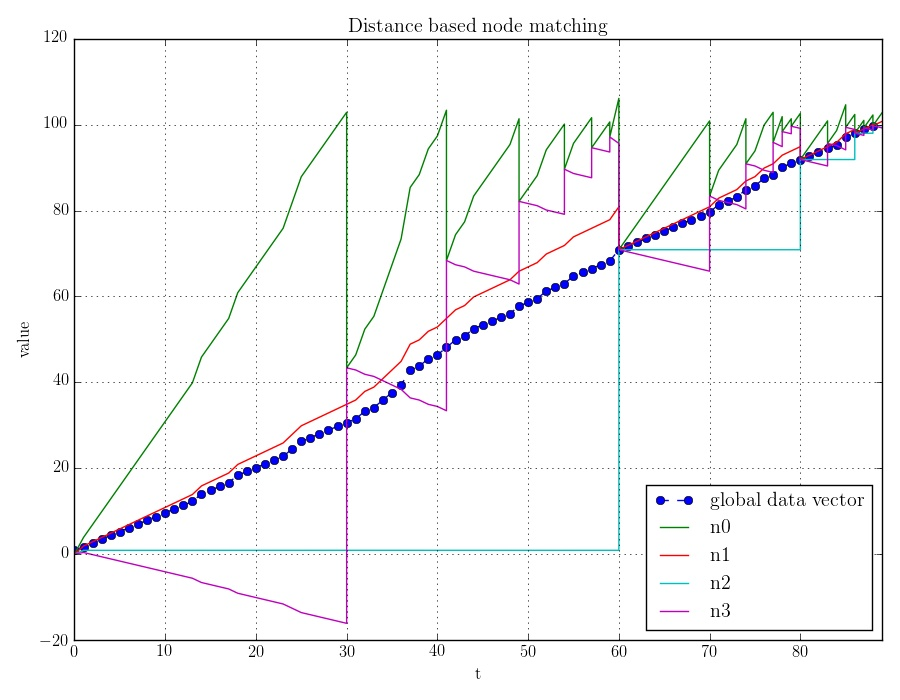
\includegraphics[scale=0.33]{img/distoptpair_example_full.jpeg}
        \caption{The drift vectors during Geometric Monitoring operation until a Global Violation. Distance based node matching is used on 4 nodes ($\{n_0, n_1, n_2, n_3\}$), with 1-dimensional data vectors, threshold $T=100$ and $f(x)=x$ as the monitoring function. The \emph{Type-2} node pairs are $\{n_0, n_3\}$ and $\{n_1, n_2\}$.}\label{fig:distoptpair}
\end{figure}
\begin{figure}
        \centering
		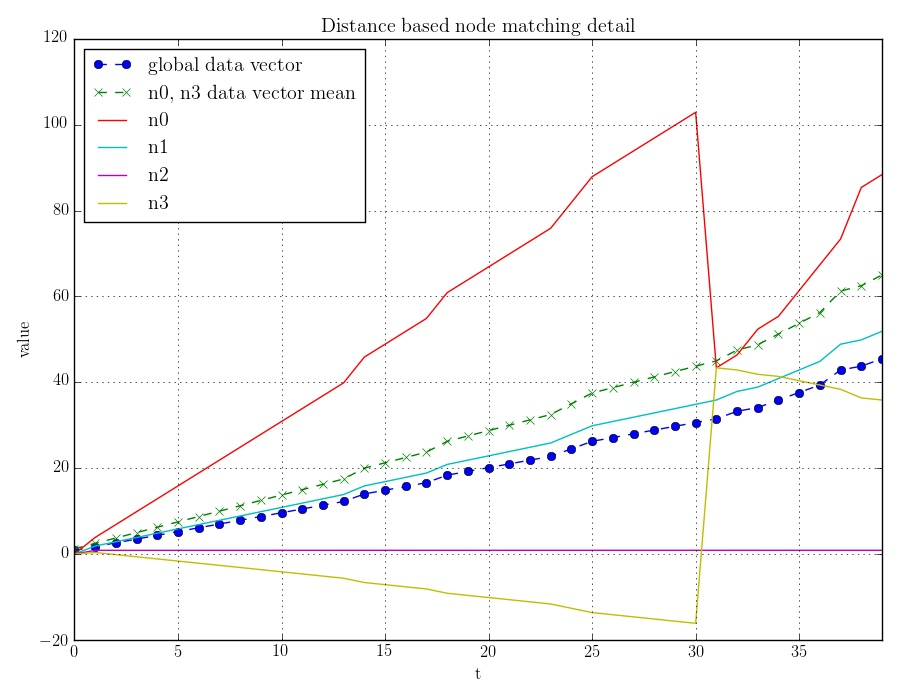
\includegraphics[scale=0.23]{img/distoptpair_example_detail.png}
        \caption{Detailed depiction of the Geometric Monitoring operation of Figure~\ref{fig:distoptpair}. Distance based node matching operating on 4 nodes ($\{n_0, n_1, n_2, n_3\}$), with 1-dimensional data vectors, threshold $T=100$ and $f(x)=x$ as the monitoring function. Distance $d_1$ denotes the distance of the data vector mean of the paired nodes $n_0$ and $n_3$ from the global mean (\emph{global data vector}) at $t=25$, whereas distance $d_2$ denotes the in-between distance of data vectors $\vec{v_0}(t)$ and $\vec{v_3}(t)$ of the node pair at time $t=25$ (before a Local Violation occurs, where $\vec{e}=0$ and $\vec{u_i}(t)=\vec{v_i}(t)\ \forall\ i\in[0,1,2,3], t<30$). Both distances are taking part in the edge weighting process, according to Equation~\ref{form:distanceMatchingWeights}.} \label{fig:distoptpairdetailed}
\end{figure}%

%%%%%%%%%%%%%%%%%%%%%%%%%%%%%%%%%%%%%%%%%%%%%%%%%%%%%%%%%%%%%%%%%%%%%%%%%%%%%%%%%%%%%%%%%%%

The incentive behind the distance based node pairing scheme comes from the need to track the global data vector as closely as possible, with only a subset of the total node population's data vectors at each balancing attempt. By considering the distance of the mean of a pair of data vectors from the global data vector (distance $d_1$ in Figure~\ref{fig:distoptpairdetailed}) the \emph{``quality''} and \emph{``accuracy''} of the tracking ability of each pair is evaluated. Additionally, by taking into account the in-between distance of data vectors of each node pair (distance $d_2$ in Figure~\ref{fig:distoptpairdetailed}), pairs from the limits of the data vector velocity spectrum that manage to \emph{``cancel each other out''} more effectively are encouraged.
\newpage
\section{Heuristic Balancing} \label{sec:impl-heuristic}
%TODO: check notes for additional stuff to add

The balancing method incorporated into the \emph{coordinator based} algorithm of the Geometric Monitoring method~\cite{Sharfman2006GM} (Section~\ref{sec:theorBack-GM}) attempts to minimize the communication overhead of local violations by computing the, so called, \emph{balancing vector}. The \emph{balancing vector} is defined as the weighted mean of the drift vectors of the nodes contained in the balancing set, and, in case of a successful balance, it is guaranteed that $B(\vec{e}, \vec{b})$ is monochromatic. Consequently, by setting the drift vectors of the nodes in the balancing set to be equal to the balance vector, all local constraints are fulfilled and the convexity property of the drift vectors is satisfied.

While this method partially succeeds in reducing the communication burden of false alarms either by requesting only a subset of the total node set each time a Local Violation occurs or by setting the drift vectors to a safe point (represented by the balance vector), major drawbacks can be noted regarding vector positioning and bounding ball construction. Updated vector assignment as a result of the ``optimization'' procedure does not take into account the idiosyncrasies of the monitoring function and the admissible region it produces. Additionally, all nodes taking part in the balancing process are handled identically, without taking advantage of the differences in the behavior of each node.

Previous work proposed selecting an optimal reference vector, instead of the estimate vector for bounding ball computation, along with shape customization of the local constraints at the nodes according to the node's needs~\cite{Sharfman2012ShapeSensGM}. Local constraint customization served as the basis for the now popular \emph{Safe-Zone} framework~\cite{Keren2013SafeZones, Keren2014GMHetStreams}, which diverges from the traditional bounding sphere setting, while maintaining the same fundamental idea of distance computation of a point from a set of support vectors~\cite{Samoladas2013Unification}, preserving the essence of the admissible region and retaining the balancing process of the coordinator based scenario.

our approach: optimaly position new drift vectors to maxinize the time until a local violation.\\
use simple velocity and acceleration estimations of drift vectors to enhance results.

the heuristic formula and explain

images of optimal positions in 2-d (3-d?)

analyze the method (bilevel multiobjective optimization), write the formulas of optimization (stackoverflow style)\\
mention solvers used 

algorithm

%%%%%%%%%%%%%%%%%%%%%%%%%%%%%%%%%%%% balancing figure %%%%%%%%%%%%%%%%%%%%%%%%%%%%%%%%%%%%
\begin{figure*}[t!]
\centering
\begin{subfigure}[t]{0.45\textwidth}
\centering
\includegraphics[scale=0.45]{img/classic_balancing.tex}
\caption{The classic balancing method. As long as $B(\vec{e}, \vec{b})$ is monochromatic (i.e. within the Admissible region), balance is successful and the updated drift vectors are set to $\vec{u_1}'=\vec{u_2}'=\vec{b}$.} 
\label{fig:classicbalancing}
\end{subfigure}
\begin{subfigure}[t]{0.45\textwidth}
\centering
\includegraphics[scale=0.45]{img/heuristic_balancing.tex}
\caption{The heuristic balancing method. Arrows depict the velocities of each drift vector. After a successful balance is achieved ($B(\vec{e}, \vec{b})$ is monochromatic), the optimal points in which the updated drift vectors ($\vec{u_1}', \vec{u_2}'$) should be positioned are computed by maximizing the estimated time until the next Local Violation, based on the current drift vector positions and the estimated velocities. Balance vector $\vec{b}$ remains unchanged.\\} 
\label{fig:heuristicbalancing}
\end{subfigure}
\caption{Balancing methods}
\end{figure*}
%%%%%%%%%%%%%%%%%%%%%%%%%%%%%%%%%%%%%%%%%%%%%%%%%%%%%%%%%%%%%%%%%%%%%%%%%%%%%%%%%%%%%%%%%%%

\subsection{Smoothing, Velocity and Acceleration Estimation via Savitzky-Golay} \label{subsec:impl-heuristic-vel}

why S-G:
smoothing and derivation at the same time\\
precomputed coefficients (real time)\\
easy implementation\\
customizable(window and order)\\

S-G implementation and algorithm\\

Example images of same data smoothed, velocity and acceleration (3 figures or all in one?)

\section{Implementation Challenges} \label{sec:impl-implChallenges}

training data\\
can be overcome, worst case scenario our algorithm operates just like the original GM

complexity of optimization (i.e. optimal point location)

complexity of optimization (i.e. node matching)
    %part
    \part{RESULTS AND CONCLUSIONS} \label{pt:resConc}
    \chapter{Experimental Results} \label{chap:expRes}

experimental result showcase

\section{Experimental Setting} \label{sec:expRes-setting}

dataset used

reference appendix for tools, mention in short

\section{Distance Based Node Matching} \label{sec:expRes-distNodeMatch}

comparison with random matching\\
comparison with distribution node matching deligiannakis\\
!use same balancing, both classic and heuristic! (i.e. 1st all with classic, then all with heuristic)
explain

\section{Heuristic Balancing} \label{sec:expRes-heuristic}

comparison with classic balancing\\
!random matching!\\
explain

how S-G affects results

\section{Overall Results} \label{sec:expRes-overall}

summarise results\\
compare classic random and classic distribution optpair with heuristic distance optpair\\
observe how S-G affects results again\\

explain
    \chapter{Conclusions and Future Work} \label{chap:concFuture}

\section{Conclusions} \label{sec:concFuture-conc}

While the geometric monitoring method and its successors provide an efficient framework for monitoring distributed data streams, prior work's experimental results indicate that the scalability of this method can be vastly improved while respecting a communication-accuracy trade-off. Aspects of the method, such as optimal local constraints at the nodes, as provided by Safe Zones~\cite{Keren2013SafeZones}, as well as deterministic selection of nodes during the balancing process~\cite{Keren2014GMHetStreams} succeed at relieving the communication burden of the monitoring task at hand.

Motivated by the aforementioned work on geometric monitoring, this thesis proposes a heuristic method to improve the original balancing process, an aspect not extensively reviewed. By employing multi-objective optimization methods, and specifically \emph{Sequential Least Squares Programming}, as well as the \emph{Savitzky-Golay smoothing and differentiating filter} for smoothing and estimating the velocity and acceleration of data stream projections, we propose a method to optimally position drift vectors during a balancing process in order to maximize the estimated time until a successive Local Violation. Furthermore, a distance-based improvement of the method for hierarchical clustering of nodes, originally proposed in~\cite{Keren2014GMHetStreams}, is presented, which clusters node pairs into disjoint sets that will effectively lead to a successful balance, while closely tracking the (unknown) global statistics stream and, at the same time, decoupling the matching operation from the monitoring function. Both of these methods are fully compatible with the original geometric monitoring method, as well as the improvements found in related work.

Evaluation on synthetic and real-world datasets retrieved from the ``European Environmental Agency - AQ e-Reporting'' database showcase the advantages and the drawbacks of our methods. When the monitoring task is compromised of smooth data streams without violent fluctuations and relatively low noise our heuristic method for node balancing, alongside our hierarchical node clustering scheme, achieves a communication reduction of up to 60\% compared to the original geometric monitoring method. On the other hand, when data streams are irregular as a function of time, or their signal to noise level is low, care must be taken at the selection of the Savitzky-Golay filter parameters for velocity and acceleration estimation of streams.


\section{Future Work} \label{sec:concFuture-future}

Multi-objective optimization and advanced solvers are able to provide optimal, or nearly optimal solutions to a variety of fields, including the area of distributed data streams. As a multitude of sophisticated solvers exist, further research directed towards the formulation of more elaborate optimizing functions regarding the balancing process of the geometric monitoring method would be a promising continuation of contemporary work on the subject. 

Regarding the estimation of velocity and acceleration of data streams in order to avert future constraint violations, sophisticated prediction models, such as multi-dimensional Gaussian processes and parameter estimation techniques for signal processing filters in the likes of the Savitzky-Golay filter provide an interesting field for exploration and experimentation on data stream systems.

    
    % Endmatter
    % For BibTeX references: specify a .bib file and a style
    % ECE dept. use USU-IEEEtran \references{sample}{USU-IEEEtran}
    % MAE dept. use aiaa or asme \references{sample}{aiaa} or
    													 % \references{sample}{asme}
    % CS dept. use \references{sample}{IEEEtran.bst}
    \references{thesis}{IEEEtran.bst}
	
	%\makeappendix
	%\appendix{Geometric Monitoring Python Implementation} \label{app:GMPI}

\appendixsection{Python} \label{appsec:GMPI-python}

what is python\\
why python

\appendixsection{Numpy and Scipy} \label{appsec:GMPI-npsp}

what are they\\
why use them and how

\appendixsection{Openopt} \label{appsec:GMPI-openopt}

what is it\\
details about framework

\appendixsection{NetworkX} \label{appsec:GMPI-nx}

what is it\\
details about framework

\appendixsection{Putting It All Together} \label{appsec:GMPI-allTogether}

code description

UML

how to run    
    %\include{vita}     % optional
    %}}}
\end{document}
